\documentclass[a4paper, 11pt]{article}
\usepackage{geometry}
\usepackage{amsfonts, epsfig}
\usepackage{amsmath}
\usepackage{wrapfig} % for wrapping text around figures and tables
\usepackage{graphicx}
\usepackage{float}
\usepackage{multirow}
\usepackage{fancyhdr}
\usepackage{booktabs} % for better table rules
\usepackage{caption} % to customize caption format
\usepackage{linegoal} % for determining the remaining width of the line
% \usepackage[backend=biber, sorting=none]{biblatex}
\usepackage[style=ieee,natbib=true,backend=biber]{biblatex}
\usepackage{subcaption}
%\usepackage{hyperref}

% reference file
\addbibresource{2489941.bib}

% custom page style
\fancypagestyle{nofooter}{
  \fancyhf{}
  \fancyhead[L]{Student Number: 2489941}
  \fancyhead[C]{Introduction to AI}
  \fancyhead[R]{\thepage}% 
  \renewcommand{\headrulewidth}{0.4pt}
}
% apply custom page style
\pagestyle{nofooter}

% redefine the table and figure formats
\captionsetup[table]{labelfont=bf}
\captionsetup[figure]{labelfont=bf, justification=centering}
\captionsetup{font=small}

\begin{document}

\begin{center}
  \subsection*{Q1 - Visualization and analysis of the Palmer penguin dataset}
\end{center}

\noindent
The Palmer penguin dataset consists of 344 records of the physical attributes of three species of penguin 
living on three islands in Antarctica (Table~\ref{tab:dataset}) \cite{PM}. In this
report, the
\begin{wraptable}{r}{0.75\textwidth} % {alignment}{width}
  \small
  \begin{center}
  \vspace{-1.7\baselineskip} % Remove space before the table
  \setlength{\abovecaptionskip}{5pt}
  \setlength{\belowcaptionskip}{5pt}
  \fontsize{10}{10}\selectfont % Change font size here
  \begin{tabular}{l|l|l|l}
  % \begin{tabular}{|p{1.8cm}|p{1.2cm}|p{4cm}|p{1.8cm}|}
  \textbf{Feature}&\textbf{Type}&\textbf{Values in the dataset}&\textbf{Importance}\\
  \hline
  island&categorial&Torgersen, Biscoe, Dream&\ \ \ 0.12 (4)\\
  bill length&numerical&32.1mm - 59.6mm&\ \ \ 0.37 (1)\\
  bill depth&numerical&13.1mm - 21.5mm&\ \ \ 0.17 (3)\\
  flipper length&numerical&172mm - 231mm&\ \ \ 0.23 (2)\\
  body mass&numerical&2700g - 6300g&\ \ \ 0.11 (5)\\
  sex&categorial&Male, Female&\ \ \ 0.01 (6)\\
  species&categorial&Adelie, Chinstrap, Gentoo&\ \ \ \ class\\
  \end{tabular}
  \vspace{-2\baselineskip} % Remove space before title
  \end{center} 
  \caption{\centering\linespread{0.8}\selectfont Palmer penguin dataset features. Importance was calculated using random forest and a ranking is shown.}
  \vspace{-2\baselineskip} % Remove space after the table
  \label{tab:dataset}
\end{wraptable}
dataset is cleaned, explored through visualization,  carefully prepared
for investigation and finally the performances of AI approaches in classifying penguin species are compared.


\vspace{\baselineskip}
\subsection*{Data cleaning}

Eleven records have missing values. 
The two missing both \textit{sex} and all numerical features were removed as imputation is unlikely to be reliable. 
A further nine records are missing only a \textit{sex} value and were considered for imputation. 
Figure~\ref{fig:sex} shows the physical 
attributes of the male and female of each species differ statistically, making it likely that imputing \textit{sex} would be reliable. Following standardisation, 
a Shapiro-Wilk test confirmed all the numerical attributes have a normal distribution \cite{shapiro1965analysis} 
and Z-tests were applied to assess the 
hypotheses that the missing \textit{sex} value is male or is female \cite{freedman2007statistics}. 
Two of the records could be imputed as male and three as female; the 
remaining four records were removed. 
The cleaned dataset has 338 records: 147 Adelie  
(74 male, 73 female), 68 Chinstrap (34 male, 34 female) and 123 Gentoo (62 male, 61 female).

\begin{figure}[!ht]
  \vspace{-0.5\baselineskip} % Remove space before figure
  \begin{minipage}{0.5\textwidth}
    \vspace{0\baselineskip} % Remove space before figure
    \centering
    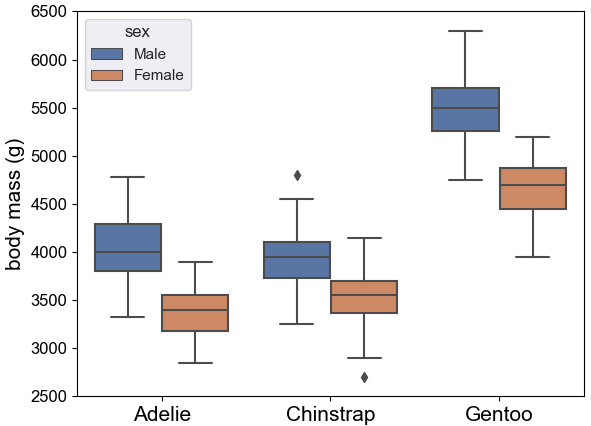
\includegraphics[width=1\textwidth]{sex.png} % Adjust the width as needed
    \vspace{-1.5\baselineskip} % Remove space before title
    \caption{All numerical features (includig body mass shown here) show a significant statistical difference between sexes}
    \vspace{-1\baselineskip} % Remove space after title
    \label{fig:sex}
  \end{minipage}\hfill
  \begin{minipage}{0.5\textwidth}
    \vspace{0\baselineskip} % Remove space before figure
    \centering
    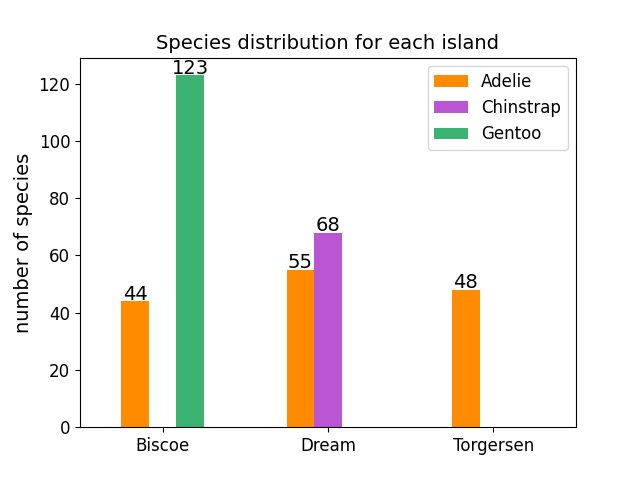
\includegraphics[width=1\textwidth]{islands.png} % Adjust the width as needed
    \vspace{-1.5\baselineskip} % Remove space before title
    \caption{Adelie is found on all three islands, but Gentoo and Chinstrap samples are found on only one of the islands}
    \vspace{-1\baselineskip} % Remove space after title
    \label{fig:islands}
  \end{minipage}
\end{figure}


% \vspace{\baselineskip}
\subsection*{Visualization of the dataset}

Figure~\ref{fig:islands} shows Chinstrap and Gentoo penguins are each found on only one of the islands, making \textit{island} a potential confounding factor since 
environmental factors may influence physical characteristics. A Shapiro-Wilk test showed  
the numerical features of the Adelie penguins (found on all the islands) have a normal distribution and an ANOVA test confirmed Adelie features are not 
significantly influenced by the island inhabited. Thus \textit{island} is unlikely to be a confounding factor.

Pairwise scatterplots for the numerical features are shown in Figure~\ref{fig:pairwise}. 
\textit{Bill depth}, combined with either \textit{flipper length} or \textit{body mass}, 
yields a separable cluster of Gentoo penguins (shown in green) allowing them to be identified. 
No pairwise combination completely separates Adelie (orange) from Chinstrap (purple) clusters, 
but the best candidate feature for doing so is \textit{bill length}.

\begin{wrapfigure}{r}{0.58\textwidth} % {alignment}{width}
  \centering
  \vspace{-1\baselineskip} % Remove space before the figure
  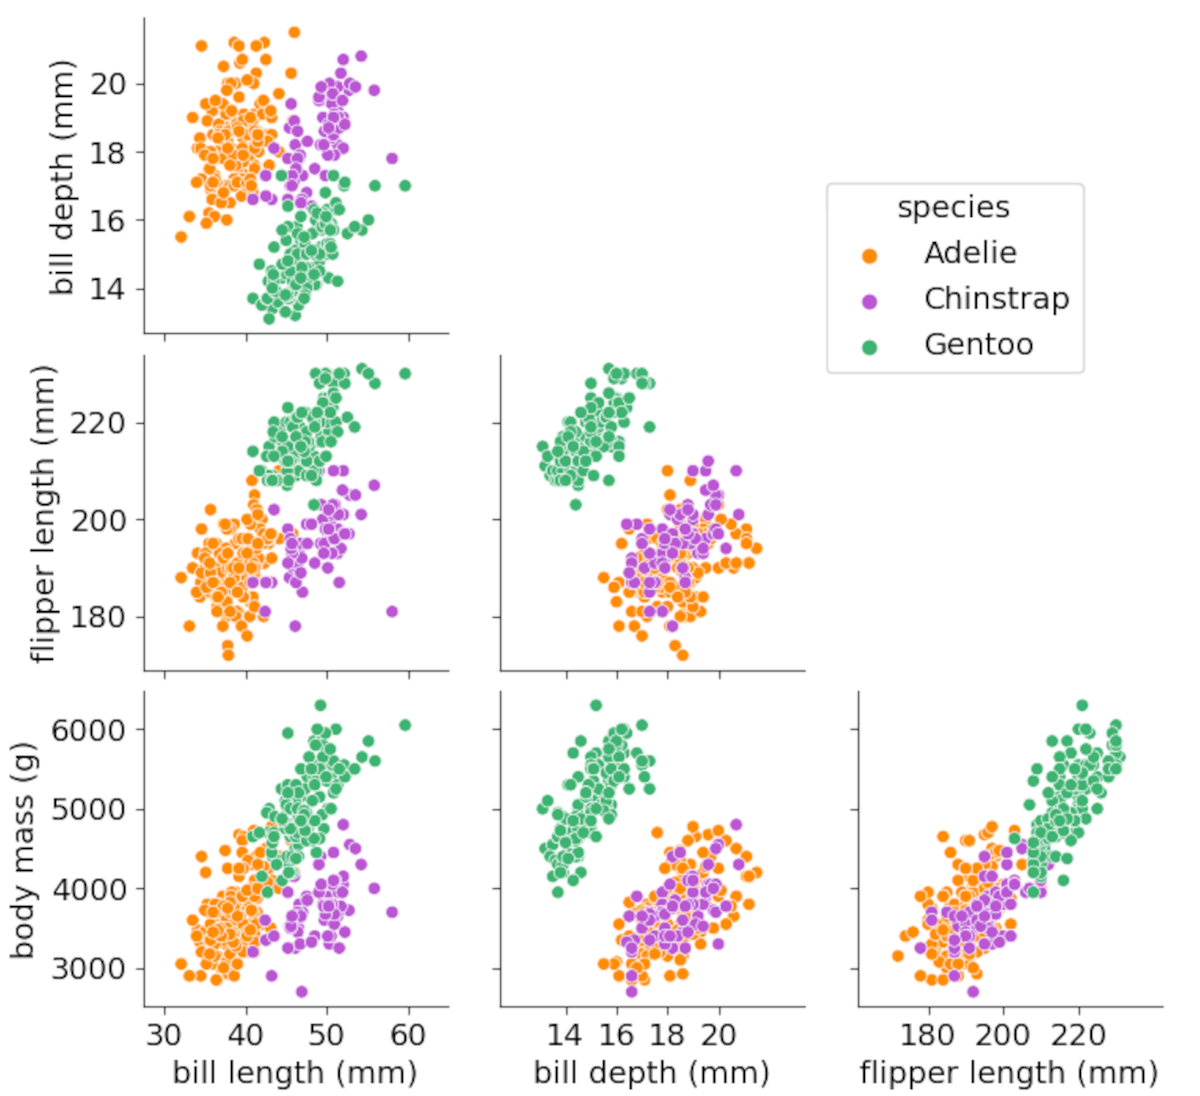
\includegraphics[width=0.58\textwidth]{pairwise.png} % Adjust the width as needed
  \vspace{-1.5\baselineskip} % Remove space before title
  \caption{\centering\linespread{0.8}\selectfont Pairwise distributions of numerical features. Gentoo can be distinguished, 
  but Adelie and Chinstrap may not be completely separable from one another}
  \vspace{-2.5\baselineskip} % Remove space after title
  \label{fig:pairwise}
\end{wrapfigure}

Figure~\ref{fig:sex} above shows the normative body masses of the male and female differ for all the species. 
Differences between the sexes for the other three numerical physical characteristics were also apparent. 
As `narrower' distributions result if the \textit{sex} of the species is considered 
rather than just the species itself, including \textit{sex} in analysis is likely to improve species classification. 
This knowledge was able to improve performance for some AI methods, as discussed in `results and analysis'.

\subsection*{Methodology}

The categorical features in the dataset were encoded to numerical values as this is required for a number of the AI methods. 
Some AI methods are known to be biased in favour of numerical features 
with smaller standard deviations \cite{hastie2009elements}, but this bias can be reduced by the standardisation 
of features to zero mean and unity standard deviation. Standardisation statistics were calculated only from 
training sets, but the standardisation itself was applied to all data, including test sets. 
If a dataset is imbalanced, AI predictions may be biased towards classes more frequently found in the training data. 
Although Adelie penguins are more populus in the dataset, all the methods adopted in the current work are known to be little affected by 
imbalanced data, so no modifications were made \cite{he2009learning}.

Predicting the penguin species from the given features is a classification problem. 
The code supporting this report is available on Github \cite{TimAIRepo}, was written in Python 3.11 \cite{python311} 
and used the \texttt{scikit-learn} libraries \cite{scikit-learn}.
Results were obtained from two conventional classification approaches, 
namely \textit{k}-Nearest Neighbour (\textit{k}nn) \cite{bishop2006pattern} and random forest \cite{breiman2001random}.
Classificaton was also carried out using 
unsupervised \textit{k}-means (following cluster labelling) \cite{tan2005introduction}, 
as well as a novel combined visualization and analysis (CVA) approach that is a mix of 
practical visualizations and Support Vector Machine (SVM) classification.

\begin{wraptable}{r}{0.6\textwidth} % {alignment}{width}
  \small
  \begin{center}
  \vspace{-0.5\baselineskip} % Remove space before the table
  \setlength{\abovecaptionskip}{5pt}
  \setlength{\belowcaptionskip}{5pt}
  \fontsize{10}{10}\selectfont % Change font size here
  \begin{tabular}{l|l|l}
  \textbf{Method} & \textbf{Metaparameters} & \textbf{Values considered}\\
  \hline
  \multirow{3}{*}{\textit{k}nn}    & nearest neighbours \textit{k}	  & \textit{\textbf{1}}, 2, 3, 4, 5, 6, 8, 10\\
                                   & prediction function	& \textit{\textbf{uniform}}, distance \\
                                   & distance metric 	& \textit{\textbf{Manhattan}}, Euclid \\
  \hline
  \multirow{6}{*}[0.5ex]{\begin{tabular}[t]{@{}l@{}}random \\ forest\end{tabular}} 
                                   & number of trees & 5, \textit{\textbf{10}}, 15, 20, 25 \\
                                   & max. depth & \textit{\textbf{no max}}, 10, 20 \\
                                   & min. samples to split  & \textit{\textbf{2}}, 5, 10 \\
                                   & min. samples at leaf & \textit{\textbf{1}}, 2, 4 \\
                                   & split function & \textit{\textbf{gini}}, entropy \\

  \hline
  \multirow{4}{*}{\textit{k}-means} & number of clusters \textit{k}  & 2, 3, \textit{\textbf{4}}, 5, 6, 7, 8, 10\\
                                    & centroid initialize         & \textit{\textbf{k-means\small{++}}}, random\\
                                    & runs for centroid	     & 2, \textit{\textbf{5}}, 10, 20 \\
                                    & max. iterations           & 5, \textit{\textbf{10}}, 20, 50 \\
  \hline
    \multirow{3}{*}{CVA}            & regularization   & 0.1, 1, \textit{\textbf{10}}, 100 \\
                                    & kernel coefficient      & \textit{\textbf{1}}, 0.1, 0.01, 0.001 \\
                                    & kernel type                  & rbf, \textit{\textbf{linear}}, poly \\
  \hline
  \end{tabular}
  \vspace{-2\baselineskip} % Remove space before title
  \end{center} 
  \caption{\centering\linespread{0.8}\selectfont Metaparameters values shown in italics most consistently produced training results of 
  best accuracy during validation and were selected for generating results}
  \vspace{-1\baselineskip} % Remove space after the table
  \label{tab:metaparameters}
\end{wraptable} 

To reduce the potential for overfitting, the classification methods were trained using 
`holdout validation', where 80\% of the dataset was used in a five-fold cross-validation 
configuration \cite{james2013introduction}. The remaining 20\% was kept for a test set. For all methods, 
the \texttt{scikit-learn} function \texttt{GridSearchCV} was employed to tune metaparameters \cite{scikit-learn}. 
The values selected for the metaparameter grid are shown in Table~\ref{tab:metaparameters} and are typical of those found in the literature \cite{geron2019hands}. 
Metaparameters giving the best 
performance were selected to generate accuracy results (the percentage of correctly predicted species) 
from the test sets. The metrics `precision' and `recall' were calculated but not included here as measures of
false positives or false negatives are not relevant to this study.

\subsection*{Results and analysis}

\begin{wraptable}{r}{0.58\textwidth} % {alignment}{width}
  \small
  \begin{center}
  \vspace{-3.5\baselineskip} % Remove space before the table
  \setlength{\abovecaptionskip}{5pt}
  \setlength{\belowcaptionskip}{5pt}
  \fontsize{10}{10}\selectfont % Change font size here
  \begin{tabular}{l|l}
  \textbf{Method} & \textbf{Accuracy (range)}\\
  \hline
  baseline, Adeleie species & 43.49\% \\
  \hline
  \textit{k}nn, all features & 99.24\% (97.06\%-100\%)\\
  \textit{k}nn, no island &	99.46\% (97.06\%-100\%)\\
  \hline
  random forest, all features	& 98.57\% (95.59\%-100\%)\\
  random forest, no body mass & 98.49\% (92.65\%-100\%)\\
  \hline
  \textit{k}-means, numerical features & 97.03\% (94.12\%-97.06\%)\\
  \textit{k}-means, two sex clusters  & 99.18\% (94.12\%-100\%)\\
  \hline
  CVA, three main features & 98.98\% (95.35\%-100\%)\\
  CVA, separate sex models & 99.25\% (90.91\%-100\%)\\
  \hline
  \end{tabular}
  \vspace{-2\baselineskip} % Remove space before title
  \end{center} 
  \caption{\centering\linespread{0.8}\selectfont Classification accuracy mean value and range for 100 pseudo-random test sets 
  and using the metaparameters identified in Table~\ref{tab:metaparameters}}
  \vspace{-1.2\baselineskip} % Remove space after the table
  \label{tab:results}
\end{wraptable} 

The \texttt{scikit-learn}  
pseudo-random procedure was used for selecting validation and test set values and 100 (indices 1 to 100) of these were used 
both when selecting metaparameters and when deriving accuracy results.
The results in Table~\ref{tab:results} include a baseline to demonstrate the 
performance improvements achieved by the AI methods. In classification, the
baseline method is often simply to select the most frequent class in the observations. Here, 
this is the Adelie penguins, giving an accuracy of 43.49\% (147/338). 

\textbf{\textit{k}nn}  
The accuracy of \textit{k}nn obtained using the dataset could be improved by removing certain features 
(particularly those shown as less important in Table~\ref{tab:dataset}).
% \begin{wrapfigure}{r}{0.46\textwidth} % {alignment}{width}
%   \centering
%   \vspace{-0.5\baselineskip} % Remove space before the figure
%   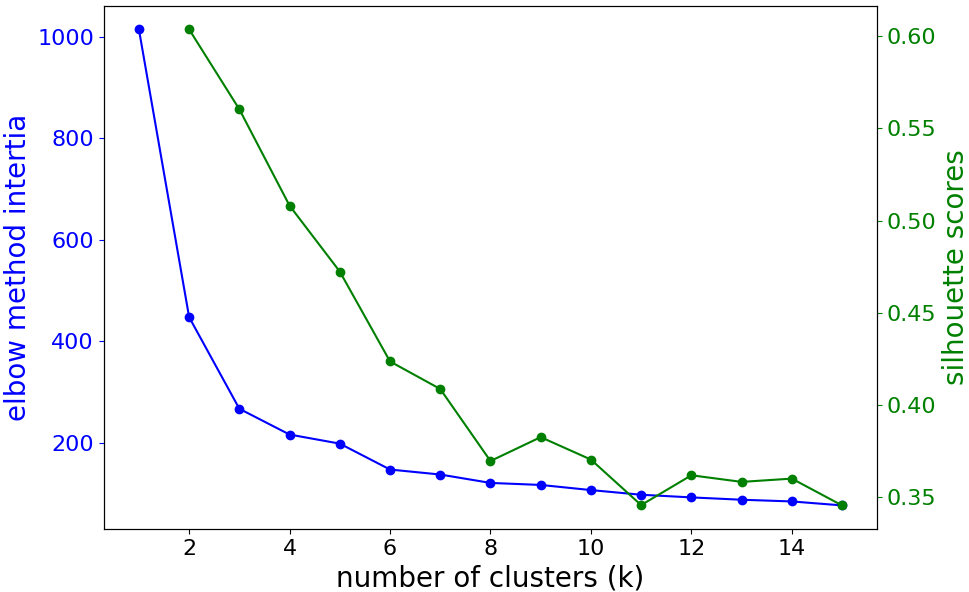
\includegraphics[width=0.48\textwidth]{kmeansvalue.png} % Adjust the width as needed
%   \vspace{-1.5\baselineskip} % Remove space before title
%   \caption{\centering\linespread{0.8}\selectfont The \textit{k}-means elbow is the change in slope of `inertia' (\textit{k}=3)
%   and the silhouette is the `score' closest to 1 (\textit{k}=2)}
%   \vspace{-1\baselineskip} % Remove space after title
%   \label{fig:kmeansvalue}
% \end{wrapfigure}
The best improvement was found when \textit{island} was omitted and when \textit{k}=3 (Table~\ref{tab:results}). It appears that \textit{island} did not provide 
any additional information and the larger value of \textit{k} (compared to \textit{k}=1 for all features) implies better generalization has been achieved during training.

\textbf{Random forest}  
When all features are inlcuded in the analysis, the accuracy of random forest was marginally worse 
than achieved using \textit{k}nn. 
No performance improvement was found using fewer features, indicating that random forest
may be less influenced by superfluous information in the training data. 

\textbf{\textit{k}-means} Although a clustering method, 
\textit{k}-means can be used for classification by 
\begin{wrapfigure}{r}{0.5\textwidth} % {alignment}{width}
  \centering
  \vspace{-0.8\baselineskip} % Remove space before the table
  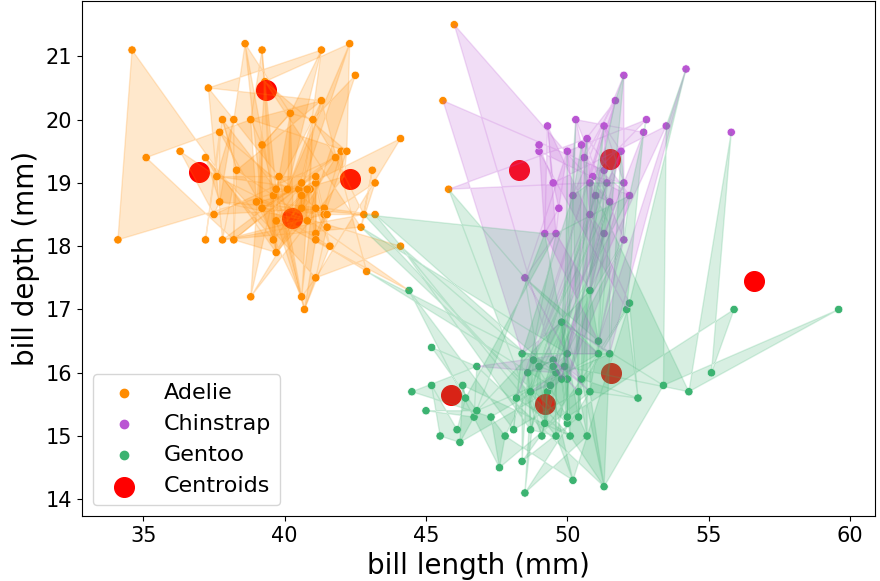
\includegraphics[width=0.48\textwidth]{kmeansmap.png} % Adjust the width as needed
  \vspace{-0.5\baselineskip} % Remove space before title
  \caption{\centering\linespread{0.8}\selectfont \textit{k}-means clusters mapped to species using majority voting. 
  Mappings are shown by polygon colour (\textit{k}=10, 50 samples included).}
  \vspace{-1\baselineskip} % Remove space after title
  \label{fig:kmeansmap}
\end{wrapfigure}
mapping clusters to classes. 
Figure~\ref{fig:kmeansmap} illustrates such a mapping for two feature dimensions.
Using the elbow method, the number of clusters (\textit{k}) was suggested to be two, but three was identified 
by the silhouette method. By trial and error, accuracy was found to improve when \(k \geq 4\),
as otherwise clusters were not reliably formed for all three species.   
Accuracy was also greatly improved by creating a separate set of clusters for each \textit{sex}.

\textbf{CVA}  
requires manual identification of suitable pairs of features for SVM classification. 
Given features \textbf{x}, SVM finds a decision boundary that maximizes class separation
\vspace{-0.8\baselineskip} % remove space before equation
\begin{equation}
\mathbf{w}^T \mathbf{x} = b ,
\end{equation}
where \textbf{w} is a weight vector perpendicular to the boundary and \textit{b} is the intercept. 
SVM training finds \textbf{w} and \textit{b} to specify an optimal hyperplane (and hence the boundary). 
An application of CVA to the Penguin dataset is given in Figure~\ref{fig:CVA}. 
Figure~\ref{fig:CVA}(a) shows the relationship between \textit{bill depth} and \textit{flipper length}, and
the SVM decision boundary separates Gentoo from the other two species. 
Figure~\ref{fig:CVA}(b) plots \textit{bill length} against \textit{bill depth} and shows the SVM boundary to best
distinguish Adelie from Chinstrap. Accuracy was improved by implementing separate SVM models for each \textit{sex}.

\begin{figure}[!ht]
    \vspace{-0.5\baselineskip} % Remove space before figure
    \begin{subfigure}{0.47\textwidth}
    \centering
    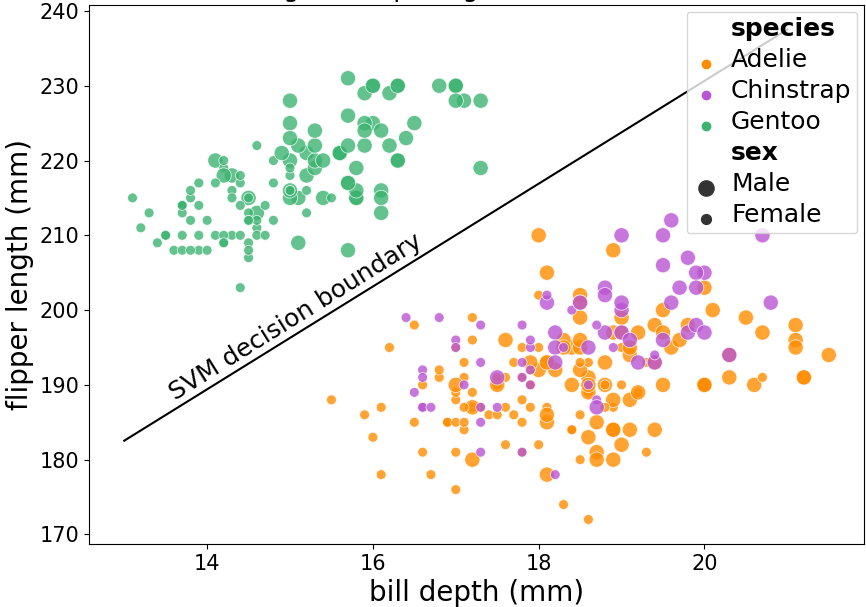
\includegraphics[width=1\textwidth]{sup_fliplen_billdepth.png} % Adjust the width as needed
    \vspace{-1.2\baselineskip} % Remove space before title
    \caption{ Gentoo distinguished from the other species}
    \vspace{-1.5\baselineskip} % Remove space before title
    \label{fig:CVA_part_a}
  \end{subfigure}
  \hfill
  \begin{subfigure}{0.47\textwidth}
    \centering
    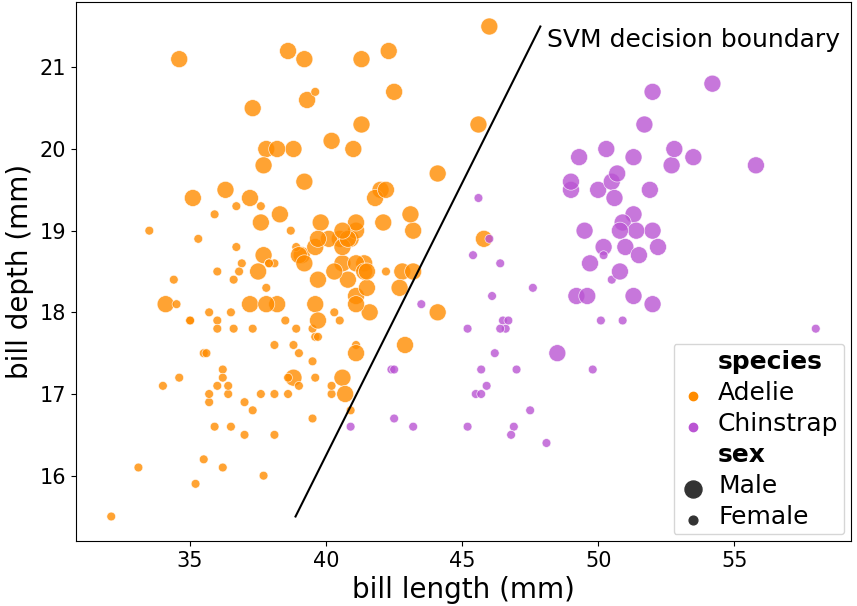
\includegraphics[width=1\textwidth]{sup_billlen_billdepth.png} % Adjust the width as needed
    \vspace{-1.2\baselineskip} % Remove space before title
    \caption{ Adelie and Chinstrap partially separated}
    \vspace{-1.5\baselineskip} % Remove space before title
    \label{fig:CVA_part_b}
  \end{subfigure}
  \vspace{1\baselineskip} % Remove space before title
  \caption{\centering\linespread{0.8}\selectfont Two-stage CVA approach with decision boundaries fitted to feature pairs using SVM}
  \label{fig:CVA}
  \vspace{-2\baselineskip} % Remove space after title
\end{figure}
\vspace{\baselineskip}

\subsection*{Conclusions}

With careful data preparation, selection of metaparameters and robust application of training and testing methods, 
\textit{k}nn and random forest both produced high-quality results. 
\textit{k}-means training does not take advantage of target information and this resulted in comparatively poor accuracy, but training
separate clusters for each sex did improve performance significantly.
The novel CVA approach needs to be tailored anew to each problem and is not well-suited to high-dimensional data, 
but it was found to produce results comparable to those of general-purpose classification methods and has the advantage that 
its internal operations are easy to visualize, understand and explain.

That CVA makes a series of decisions using chosen feature pairs 
led the author to consider SVMs in place of entropy at random forests nodes - 
but this has been done \cite{law2003support}!

\vspace{-0.1\baselineskip} % Remove space before figure
\begin{center}
\subsection*{Question 2 - Ethical challenges and threats in AI}
\end{center}
\vspace{0.1\baselineskip} % Remove space before figure
\subsection*{Racial Bias in Medical Algorithms}

In 2019, a widely used US healthcare algorithm was found to discriminate by prioritising hospital services 
based on historical spending records, resulting in the allocation of relatively less future funding and fewer referrals 
for black patients \cite{Jemielity2019, Ledford2019}. 
Through the application of a series of test data sets, Obermeyer \textit{et al.} \cite{Obermeyer2019} identified this inadvertent bias 
and the team was able to mitigate against it by adjusting the model’s training labels. 

The fact that this third-party assessment and adjustment were possible, demonstrates how exposing a model’s internal operations 
can aid bias identification and removal \cite{Seroussi2020, Winter2023}. 
Ensuring greater transparency of AI models is becoming the subject of legislation, 
for example the 2023 EU AI Act aims to enforce transparency principles by requiring developers to disclose an 
algorithm’s variables, data sources, and selection logic \cite{EuropeanParliament2023, Edwards2021}. 
While ensuring that organisations building AI systems are held accountable for the processes used in their development 
may lead to algorithmic changes that reduce bias \cite{Donovan2018, Lawry2020}, 
care needs to be taken that the removal of bias doesn't significantly affect the performance of the model 
in its application domain \cite{Kearns2020}.

\subsection*{AI system safety and existential risks in warfare}

Recent developments in AI have led many researchers to believe that AI systems capable of directly acting 
in the real world based on decisions they have taken autonomously will become available later this century \cite{Grace2018}. 
With such advancements comes the risk that AI systems whose decision-making does not prioritise human welfare 
may pose a threat to life \cite{Ord2020}. 

A specific example of a military AI system posing an existential risk \cite{yampolskiy2016, Cummings2017}, 
is one that decides maximising human casualties would be the best strategy to achieve a high-level battlefield objective \cite{Barrat2013}. 
Recent deployments of automated missiles that activate on target acquisition \cite{Atherton2021, BodeWatts2023}, 
have raised ethical concerns over the use of AI in situations where human beings are potential targets \cite{Emery2021}. 
If such advanced AI was given control of powerful military weapons and applied more widely, 
the ramifications for the human race's survival could be profound \cite{Tegmark2017}. 

Addressing these existential threats requires international cooperation 
to guarantee the transparency of AI algorithms \cite{Cihon2019, Leslie2019}. 
A potential future safeguard is to include a human-controlled override in all military AI systems \cite{CritchKrueger2020}, 
although Russell \cite{Russell2019} warns that super-intelligent AI may be capable of removing such safety measures. 
Ultimately, a global strategy that prioritises human wellbeing in all areas of AI usage will be essential.

\printbibliography
\end{document}
